%%%%%%%%%%%%%%%%%%%%%%%%%%%%%%%%%%%%%%%%%
% Stylish Article
% LaTeX Template
% Version 2.1 (1/10/15)
%
% This template has been downloaded from:
% http://www.LaTeXTemplates.com
%
% Original author:
% Mathias Legrand (legrand.mathias@gmail.com) 
% With extensive modifications by:
% Vel (vel@latextemplates.com)
% Final ACS by:
% Juan Barbosa
% License:
% CC BY-NC-SA 3.0 (http://creativecommons.org/licenses/by-nc-sa/3.0/)
%
%%%%%%%%%%%%%%%%%%%%%%%%%%%%%%%%%%%%%%%%%
\documentclass[fleqn,11pt]{SelfArx}
%\usepackage[superscript]{cite}
\usepackage{wrapfig}
\usepackage{rotating}
\usepackage{subcaption}
\usepackage[numbers, super]{natbib}
%----------------------------------------------------------------------------------------
%	ARTICLE INFORMATION
%----------------------------------------------------------------------------------------

\JournalInfo{Laboratorio Org\'anica 3, No. 4, 14/10/2017} % Journal information
\Archive{ }

\PaperTitle{Acilación de Friedel-Crafts} %
%\Keywords{Keyword1 --- Keyword2 --- Keyword3} % Keywords - if you don't want any simply remove all the text between the curly brackets
%\newcommand{\keywordname}{Keywords} % Defines the keywords heading name

%----------------------------------------------------------------------------------------
%	ABSTRACT
%----------------------------------------------------------------------------------------

\Abstract{
\begin{wrapfigure}{r}{0.45\textwidth}
	\centering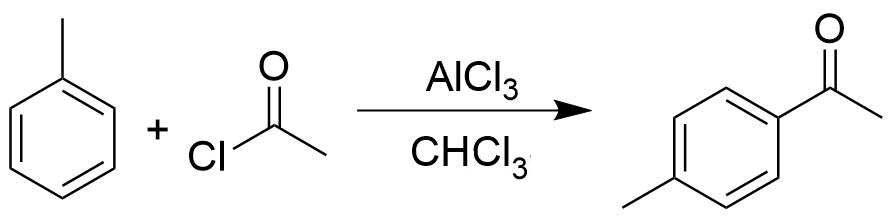
\includegraphics[width=0.95\linewidth]{structures/reaction.png}
\end{wrapfigure}

La preparación del 4-metilacetofenona se llevó a cabo usando tolueno, cluroro de acetilo, y cloruro de aluminio (III) como ácido de Lewis, en una reacción de acilación de Friedel-Crafts, usando cloroformo como disolvente. La reacción tuvo una duración de 2 horas y un rendimiento de \_\_\_ \%, sin requerir un tratamiento de purificación. La caracterización del producto se llevó a cabo usando $^1$HRMN y $^{13}$CRMN.
}

%----------------------------------------------------------------------------------------

\begin{document}

\flushbottom % Makes all text pages the same height

\maketitle % Print the title and abstract box

%\tableofcontents % Print the contents section

\thispagestyle{empty} % Removes page numbering from the first page
\renewcommand{\tablename}{Tabla} 


%----------------------------------------------------------------------------------------
%	ARTICLE CONTENTS
%----------------------------------------------------------------------------------------

\section*{Introducci\'on} % The \section*{} command stops section numbering
%------------------------------------------------
Dos reacciones llevan el nombre de los químicos Charles Friedel y James Crafts, ambas reacciones se caracterizan por usar carbocationes como electrófilos capaces de sustituir anillos aromáticos, produciendo un nuevo enlace carbono-carbono. La primera de estas reacciones es la alquilación, en donde un cloruro de alquilo sustituye un hidrógeno de un anillo aromático activado, esto es un anillo con una alta densidad electrónica, en presencia de un ácido de Lewis para formar alquilbecenos. La segunda reacción procede de forma análoga, salvo que se hace uso de un cloruro de acilo para obtener fenil cetonas \cite{Wade2013}.
\begin{scheme}[h]
	\centering
	\caption{A la izquierda una reacción de alquilación, a la derecha acilación de Friedel-Craft. \ce{X = Cl, Br, I}, \ce{R = alquil, aril} \cite{Wade2013}.}
	\includegraphics[width=1.\linewidth]{structures/FriedelCraft.png}
\end{scheme}
\newpage

Una diferencia importante entre la alquilación y la acilación es la cantidad de ácido de Lewis requerido en la reacción, mientras en la primera se requieren cantidades catalíticas, en la acilación es necesario el uso de un equivalente. A pesar de esto la acilación es considerablemente más usada experimentalmente porque no permite que la reacción se lleve a cabo más de una vez. Esto se debe a que el producto de la reacción es una cetona, donde se tiene unido al anillo un grupo carbonilo, el cual extrae carga, desactivando el mismo. Lo anterior no ocurre con alquilación por lo cual es posible obtener productos polialquilados \cite{Wade2013, sartori_maggi_2010}.

Por estas razones la acilación de Friedel-Crafts se considera un pilar fundamental en la química orgánica sintética, existen al menos 20 mil referencias que involucren esta reacción. Las cetonas aromáticas obtenidas constituyen importantes intermediarios en productos farmaceúticos, y agroquímicos, entre otros. Por ejemplo la \textit{ortho}-hidroxiacetofenona constituye un importante precursor en la síntesis de la 4-hidroxicumarina, el cual se obtiene por la reacción de fenol con ácido acetico o anhídrido acético \citealp{sartori_maggi_2010, davenport1986process}.

\begin{scheme}
	\centering
	\caption{Obtención de la \textit{ortho}-hidroxiacetofenona usando una reacción de Friedel-Crafts con \'acido acético como generador del carbocatión \citealp{davenport1986process}.}
	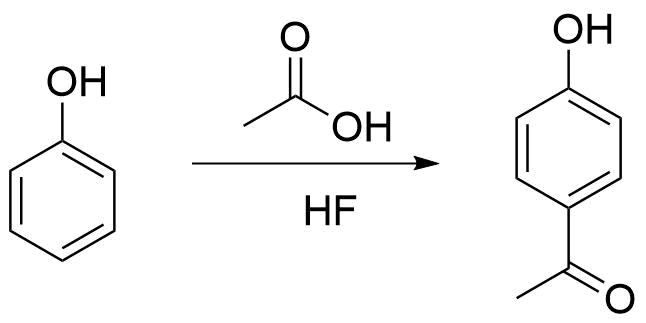
\includegraphics[width=0.7\linewidth]{structures/hidroxiacetofenona.png}
\end{scheme}


\begin{scheme*}[h]
	\centering
	\caption{Complejo sigma. Las estructuras en azul son particularmente estables por el efecto inductivo del metilo, además de tener carbocationes terciarios.}
	\includegraphics[width=0.7\linewidth]{structures/SigmaComplex.png}
\end{scheme*}

\begin{figure*}[h]
	\centering
	\begin{tabular}{ccc}
		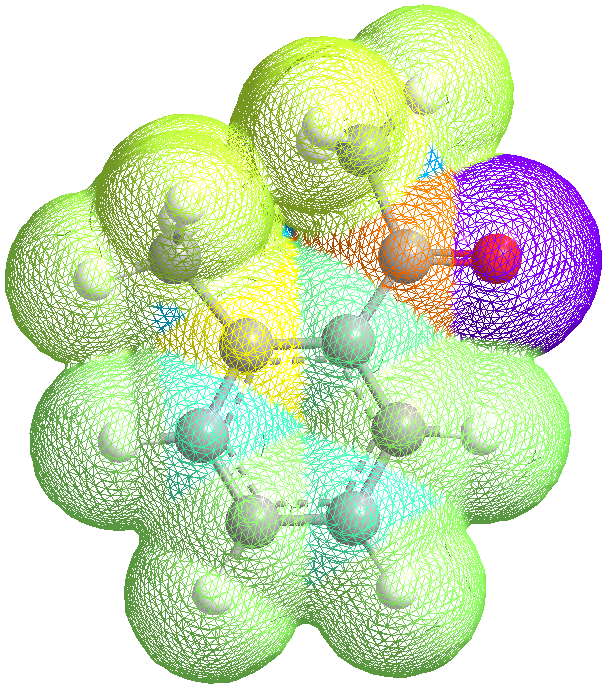
\includegraphics[width=0.3\linewidth]{structures/ortho.png} & 
		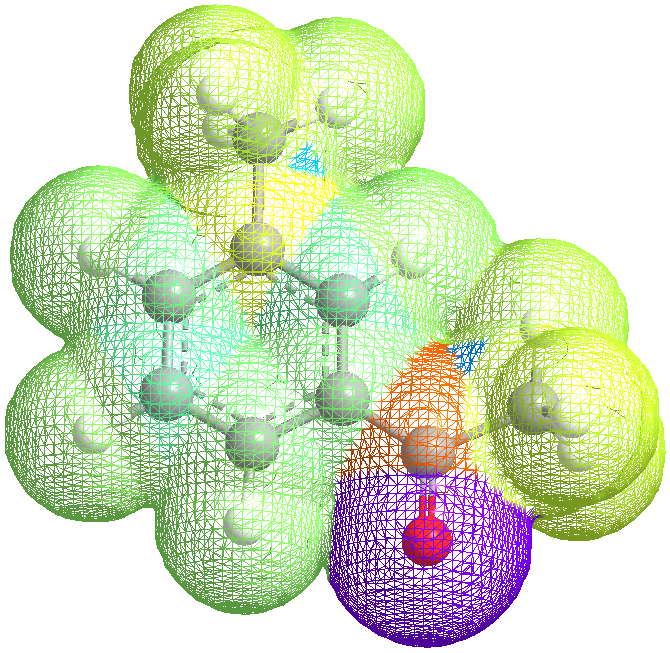
\includegraphics[width=0.3\linewidth]{structures/meta.png} &
		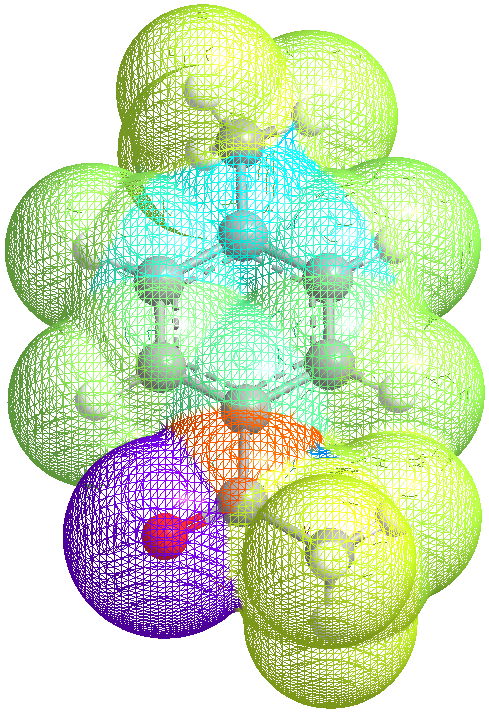
\includegraphics[width=0.25\linewidth]{structures/para.png}
	\end{tabular}
	
	\caption{Moléculas aciladas en las posiciones \textit{ortho}, \textit{meta}, y \textit{para} correspondientemente. Las energias de MM2 (\textit{Mining-Minima}) son: 14.49 kcal/mol, 8.99 kcal/mol, 8.83 kcal/mol.}
\end{figure*}

\newpage
\section{Resultados y Discusi\'on}
\section{Conclusiones}

\section{Secci\'on experimental}

%----------------------------------------------------------------------------------------
%	REFERENCE LIST
%----------------------------------------------------------------------------------------
%\newpage
\phantomsection
\bibliography{informe}
\bibliographystyle{achemso}

%----------------------------------------------------------------------------------------
\onecolumn
\section{Informaci\'on suplementaria}\label{sec: complementaria}
\end{document}